\subsection{Experimentación}

Para medir empiricamente la eficiencia del algoritmo decidimos tomar varias instancias del problema con grafos G cuya cantidad de nodos (n) va desde 5 a 200. Los grafos generados tendrán n/2-1 fábricas y n-n/2-1 clientes de manera que se cumple que la cantidad de fábricas sea menor a la de clientes. Además, la cantidad de aristas será (n(n-1))/2 lo cual nos forma grafos completos. Graficamos los resultados de los ciclos insumidos en función del número de aristas presentes en el grafo. Los resultados obtenidos fueron los siguientes:

\begin{figure}[H]
\center
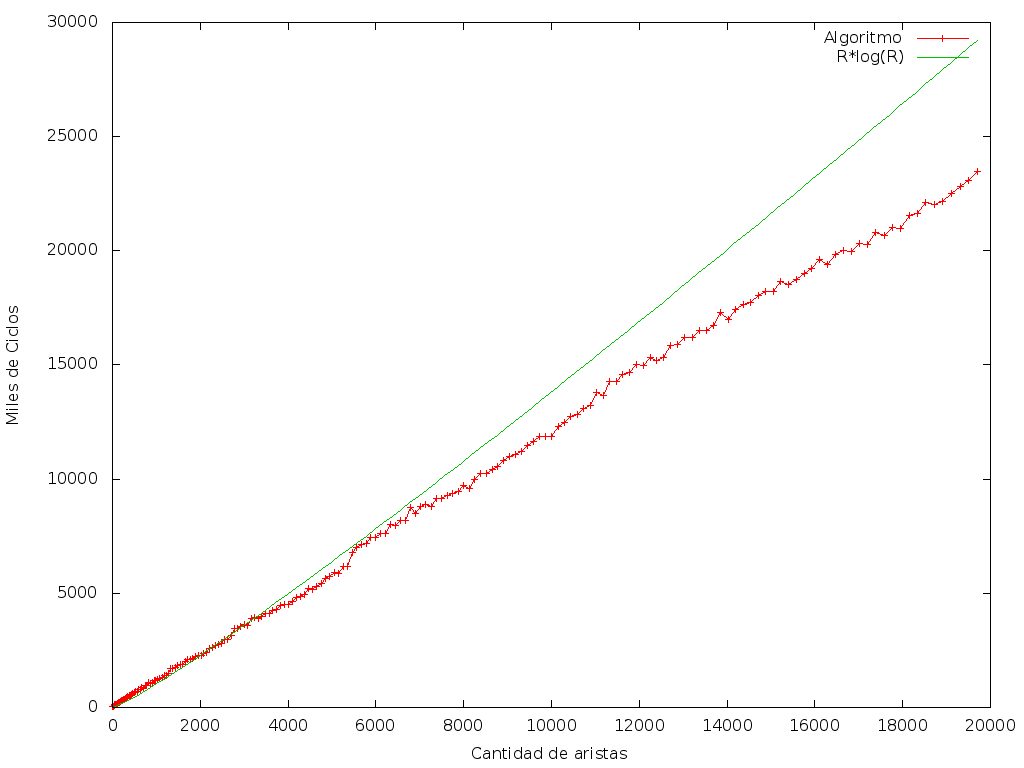
\includegraphics[scale=0.40]{ej3/imgs/complejidad.png}
\caption[Long caption]{Gráfico de complejidad para grafos completos que van desde 5 a 200 nodos.}
\label{pic-a}
\end{figure}

Como fue mencionado en la sección 4.3 (Implementación y complejidad), O(log(R))=O(log($(C+F)^2$))$\subset$ log($C^2$)=O(2 log C)$\subset$ O(log C) por lo cual mostrar que se encuentra acotado por Rlog(R) es equivalente a hacerlo por Rlog(C). Como el gráfico es de dos dimensiones, no podemos incluir la variable C al gráfico por lo cual sólo graficamos en función de la cantidad de aristas.

Viendo el gráfico podemos apreciar que el algoritmo se encuentra acotado por O(Rlog(R)) como pedía el enunciado.


